\chapter{Klassenbeschreibungen}
\minitoc

Die Klassen und deren Zusammensetzung als Gesamtsystem wird
nachfolgend beschrieben. 
\\

Angefangen mit einem Klassendiagramm unseres Plugins sowie 
dann die Gruppierung der Klassen sowie anderer Plugin Bestandteile in
Komponenten.		
\\

Tablogik: class.ilACOPlugin, class.ilACOUIHookGUI 

Gruppenerstellen: class.ilACOGroupGUI

Gruppenfilter: class.ilACOTutorGUI

Verlinkung: class.ilACOLinkGUI, class.ilACOExerciseMemberTableGUI, templates

Gruppen verwalten: class.ilACOGroupDisplayGUI

Mitgliederverschieben: class.ilACOMemberGUI

Lang Files: lang


\begin{figure}
	\centering
	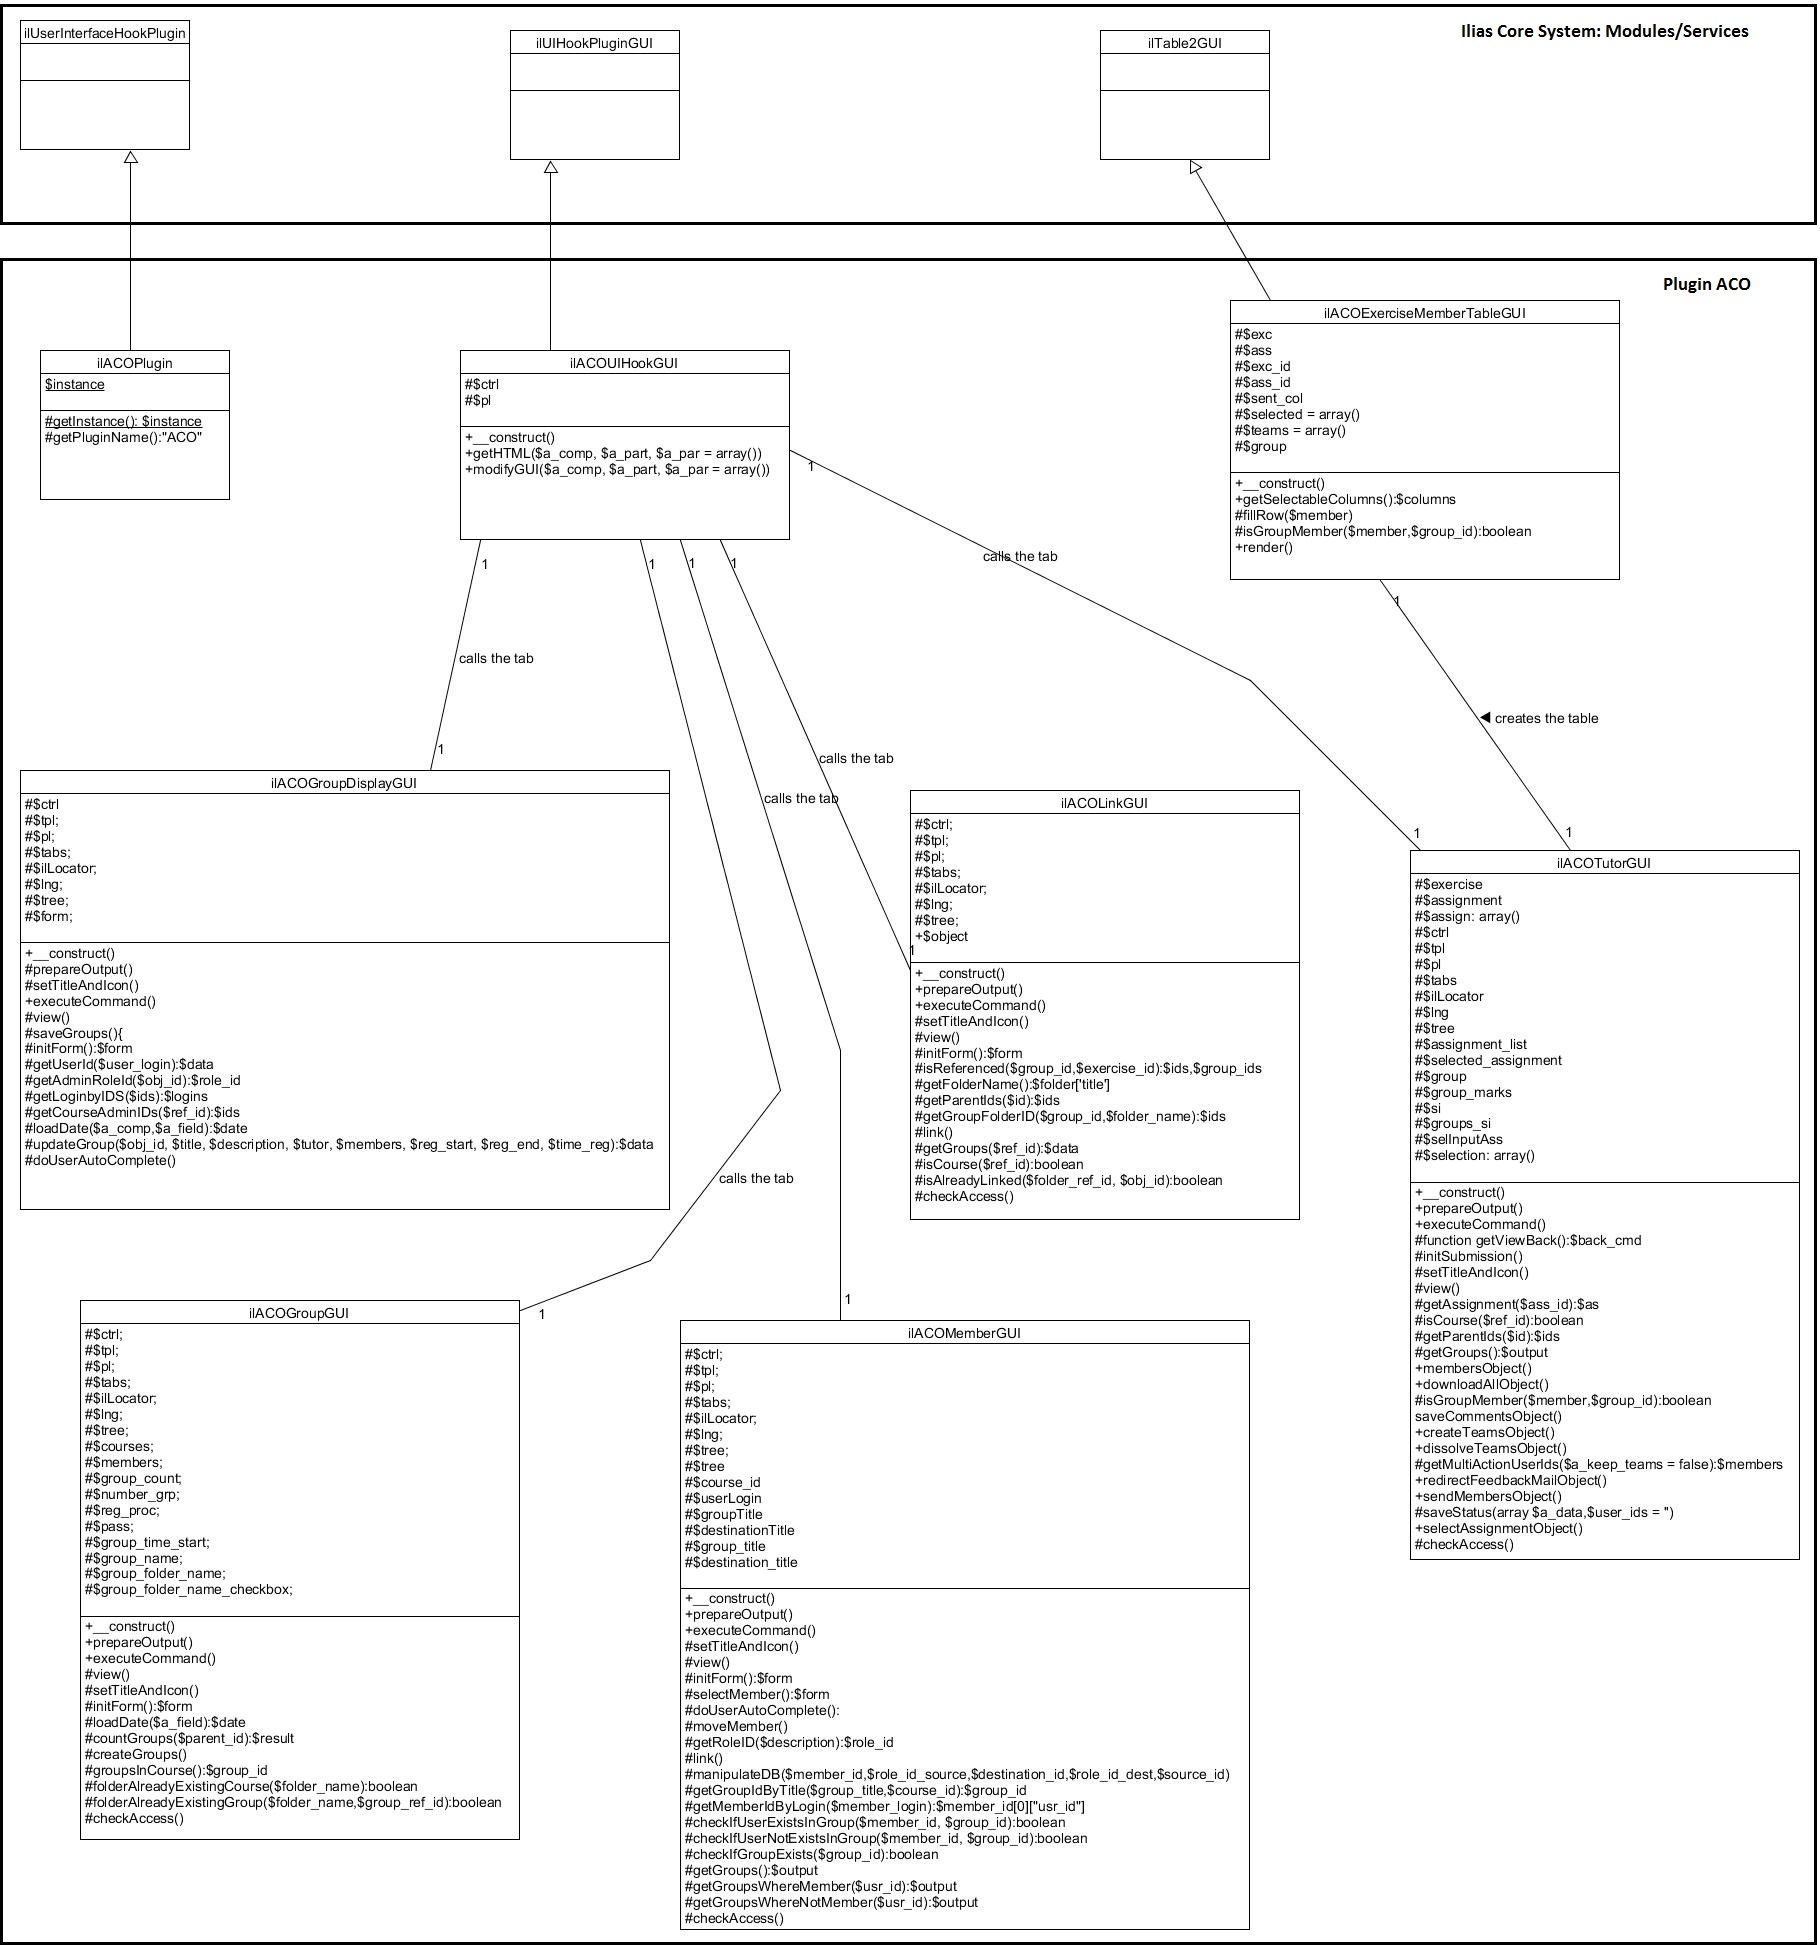
\includegraphics[width=1\textwidth]{img/klassendiagramm.jpg}
	\caption{Klassendiagramm}
\end{figure}

\newpage



\begin{figure}
	\centering
	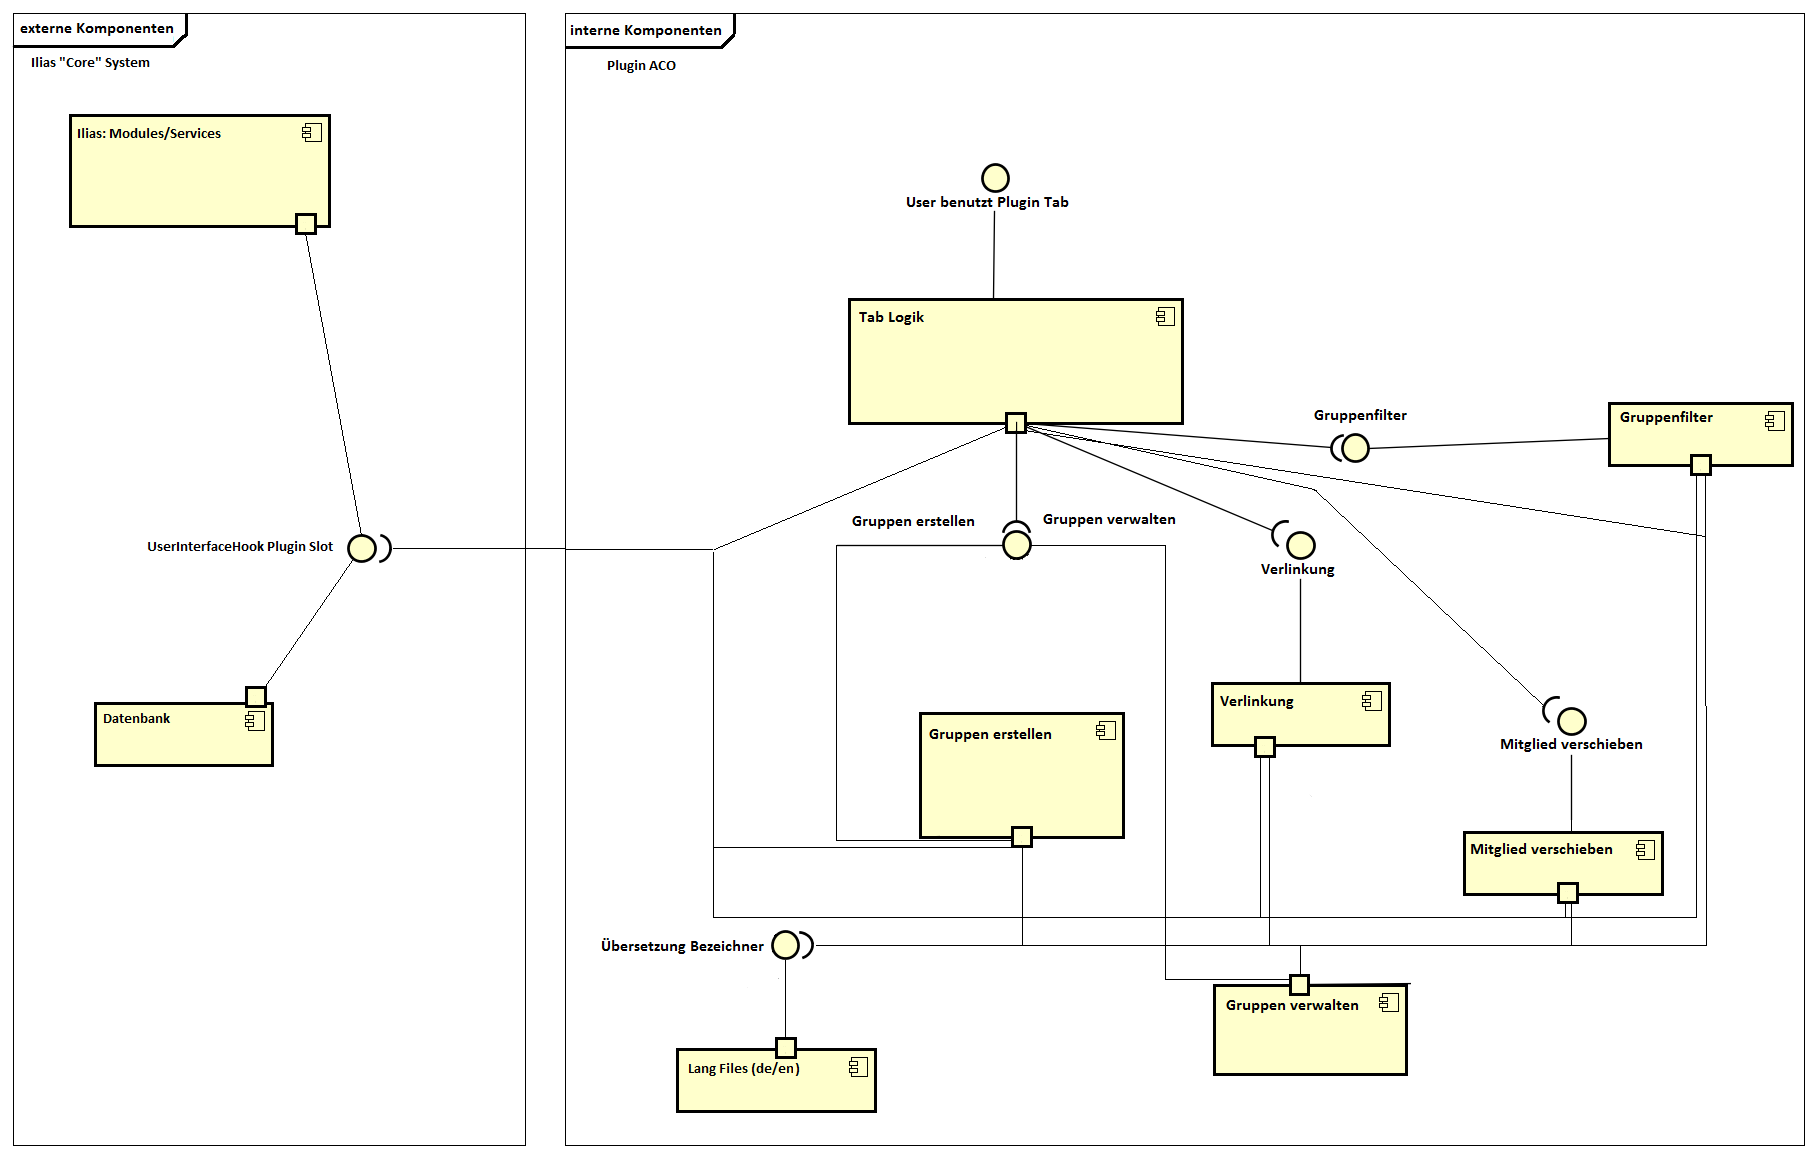
\includegraphics[width=1\textwidth]{img/ComponentDiagram.png}
	\caption{Komponentendiagramm}
\end{figure}


\clearpage


\section{ilACOExerciseMemberTableGUI}

\subsection*{Beschreibung}
Diese Klasse implementiert den Aufbau der Tabelle im Tab \textit{Gruppenfilter}. 
Sie erbt von der ILIAS-Core Klasse ilTable2GUI.

\subsection*{Klassenvariablen}
\subparagraph{exc}
protected - type: ilExercise - Die darzustellende Exercise
\subparagraph{ass}
protected - type: ilAssignment - Das darzustellende Assignment
\subparagraph{exc\_id}
protected - type: integer - ID der Exercise
\subparagraph{ass\_id}
protected - type: integer - ID des Assignment
\subparagraph{sent\_col}
protected - type: boolean - Ob eine Mail versendet wurde
\subparagraph{selected}
protected - type: Array - Selektierte Reihen
\subparagraph{teams}
protected - type: Array
\subparagraph{group}
protected - type: integer - Gruppen ID der darzustellenden Gruppe


\subsection*{Funktions-Liste}

\subparagraph{\nameref{constructEMT}}
\subparagraph{\nameref{getSelectableColumnsEMT}}
\subparagraph{\nameref{fillRowEMT}}
\subparagraph{\nameref{isGroupMemberEMT}}

\subsection*{Funktionen}

\subsubsection*{\textit{\_\_construct}}\label{constructEMT}
\subparagraph{Beschreibung}
\begin{itemize}
	\item[] \noindent\fbox{\_\_construct(\$a\_parent\_obj, \$a\_parent\_cmd, \$a\_exc, \$a\_ass,\$group\_id)}
	\item[] Konstruktor der Tabelle für \textit{Gruppenfilter}. Erstellt eine gefilterte Tabelle nach den übergebenen Parametern
\end{itemize}
\subparagraph{Parameter-Liste}
\begin{itemize}
	\item[] \textbf{a\_parent\_obj} - type: object - Objekt in dem die Tabelle erzeugt wird
	\item[] \textbf{a\_parent\_cmd} - type: String - Letztes Command der Klasse die den Konstruktor aufruft
	\item[]\textbf{a\_exc} - type: ilExercise - Exercise die in der Tabelle dargestellt werden soll
	\item[]\textbf{a\_ass} - type: ilAssignment - Assignment nach dem gefiltert wird
	\item[]\textbf{group\_id} - type: integer - Gruppen-ID nach der gefiltert wird
\end{itemize}

\subsubsection*{\textit{getSelectableColumns}}\label{getSelectableColumnsEMT}
\subparagraph{Beschreibung}
\begin{itemize}
	\item[] \noindent\fbox{getSelectableColumns()}
	\item[] Gibt ein Array zurück, welches bestimmt welche Spalten in der Tabellenansicht aktiviert bzw. deaktiviert werden können.
\end{itemize}
\subparagraph{Rückgabewerte}
\begin{itemize}
	\item[] Gibt ein mehrdimensionales Array zurück.
\end{itemize}

\subsubsection*{\textit{fillRow}}\label{fillRowEMT}
\subparagraph{Beschreibung}
\begin{itemize}
	\item[] \noindent\fbox{fillRow(\$member)}
	\item[] Füllt eine Reihe mit den Daten des übergebenen Parameter. Wird von der Methode \nameref{constructEMT} aufgerufen.
\end{itemize}
\subparagraph{Parameter-Liste}
\begin{itemize}
	\item[] \textbf{member} - type: Array - Ein Array mit den Feldern usr\_id, team\_id, team, und name
\end{itemize}

\subsubsection*{\textit{isGroupMember}}\label{isGroupMemberEMT}
\subparagraph{Beschreibung}
\begin{itemize}
	\item[] \noindent\fbox{isGroupMember(\$member,\$group\_id)}
	\item[] Überprüft auf Gruppenmitgliedschaft 
\end{itemize}
\subparagraph{Parameter-Liste}
\begin{itemize}
	\item[] \textbf{member} - type: Array - Ein Array mit minimum dem Feld usr\_id
	\item[] \textbf{group\_id} - type: integer - Gruppen-ID die überprüft wird
\end{itemize}
\subparagraph{Rückgabewerte}
\begin{itemize}
	\item[] boolean - \textbf{TRUE} falls die User-ID in der Gruppe mit der Gruppen-ID vorhanden ist, \textbf{FALSE} sonst.
\end{itemize}

\newpage
\section{ilACOGroupDisplayGUI}

\subsection*{Beschreibung}
Diese Klasse implementiert die Funktion \textit{Kurs bearbeiten} und beinhaltet die Möglichkeit, die einzelnen Gruppen in einem Kurs zentral zu verwalten. 
Hierzu werden bestimmte Parameter der Gruppen in einer tabellarischen Übersicht dargestellt und können editiert werden.

\subsection*{Klassenvariablen}
\subparagraph{ctrl}
protected - type: ilCtrl - Steuerung Zugriffsrechte
\subparagraph{tpl}
protected - type: ilTemplate - Template für Darstellung und Formatierung
\subparagraph{pl}
protected - type: ilACOPlugin - Instanz des Plugins
\subparagraph{tabs}
protected - type: ilTabsGUI - Verwaltung von Tabs
\subparagraph{ilLocator}
protected - type: ilLocatorGUI - Darstellung in der Tree Hierarchie
\subparagraph{lng}
protected - type: ilLanguage - Einbindung der Language-File von ILIAS
\subparagraph{tree}
protected - type: ilTree - Verwaltung der Tree Hierarchie
\subparagraph{form}
protected - type: ilPropertyFormGUI - Instanz eines Formulars
\subparagraph{groupAdmins}
protected - type: array - Array mit allen Admins in einer Gruppe

\subsection*{Funktions-Liste}
\subparagraph{\nameref{constructGDGUI}}
\subparagraph{\nameref{prepareOutputGDGUI}}
\subparagraph{\nameref{setTitleAndIconGDGUI}}
\subparagraph{\nameref{executeCommandGDGUI}}
\subparagraph{\nameref{viewGDGUI}}
\subparagraph{\nameref{initFormGDGUI}}
\subparagraph{\nameref{saveGroupsGDGUI}}
\subparagraph{\nameref{getUserIdGDGUI}}
\subparagraph{\nameref{getAdminRoleIdGDGUI}}
\subparagraph{\nameref{getLoginbyIDSGDGUI}}
\subparagraph{\nameref{getCourseAdminIDsGDGUI}}
\subparagraph{\nameref{loadDateGDGUI}}
\subparagraph{\nameref{updateGroupGDGUI}}
\subparagraph{\nameref{getTableDataGDGUI}}
\subparagraph{\nameref{doUserAutoCompleteGDGUI}}
\subparagraph{\nameref{checkAccessGDGUI}}

\subsection*{Funktionen}

\subsubsection*{\textit{\_\_construct}}\label{constructGDGUI}
\subparagraph{Beschreibung}
\begin{itemize}
	\item[] \noindent\fbox{\_\_construct()}
	\item[] Konstruktion der Grundinstanz
\end{itemize}

\subsubsection*{\textit{prepareOutput}}\label{prepareOutputGDGUI}
\subparagraph{Beschreibung}
\begin{itemize}
	\item[] \noindent\fbox{prepareOutput()}
	\item[] Grundlegende Eigenschaften werden festgelegt: Tabs, Position in der Tree Hierarchie, BackTarget, Titel und Icon, sowie das verwendete Template
\end{itemize}

\subsubsection*{\textit{setTitleAndIcon}}\label{setTitleAndIconGDGUI}
\subparagraph{Beschreibung}
\begin{itemize}
	\item[] \noindent\fbox{setTitleAndIcon()}
	\item[] Titel und Symbol des Objekt werden festgelegt
\end{itemize}

\subsubsection*{\textit{executeCommand}}\label{executeCommandGDGUI}
\subparagraph{Beschreibung}
\begin{itemize}
	\item[] \noindent\fbox{executeCommand()}
	\item[] Regelung der Umsetzung von Befehlen mittels CommandButtons
\end{itemize}

\subsubsection*{\textit{view}}\label{viewGDGUI}
\subparagraph{Beschreibung}
\begin{itemize}
	\item[] \noindent\fbox{view()}
	\item[] Ausgabe der initialen Ansicht als HTML-Dokument
\end{itemize}

\subsubsection*{\textit{initForm}}\label{initFormGDGUI}
\subparagraph{Beschreibung}
\begin{itemize}
	\item[] \noindent\fbox{initForm()}
	\item[] Formular wird generiert und mit initialen Werten gefüllt
\end{itemize}
\subparagraph{Rückgabewerte}
\begin{itemize}
	\item[] \textbf{form} - Formular mit Standardwerten, type: ilPropertyFormGUI
\end{itemize}

\subsubsection*{\textit{saveGroups}}\label{saveGroupsGDGUI}
\subparagraph{Beschreibung}
\begin{itemize}
	\item[]  \noindent\fbox{saveGroups()} 
	\item[] Die Änderungen in der tabellarischen Übersicht der Gruppen werden an die Funktion \nameref{updateGroupGDGUI} übergeben. Anschließend wird die tabellarische Übersicht aktualisiert, um die aktuellen Daten anzuzeigen.
\end{itemize}

\subsubsection*{\textit{getUserId}}\label{getUserIdGDGUI}
\subparagraph{Beschreibung}
\begin{itemize}
	\item[]  \noindent\fbox{getUserId(\$user\_login)} 
	\item[] Benutzername als Eingabe liefert die dazugehörige UserID
\end{itemize}
\subparagraph{Parameter-Liste}
\begin{itemize}
	\item[] \textbf{user\_login} - Benutzername, type: String
\end{itemize}
\subparagraph{Rückgabewerte}
\begin{itemize}
	\item[] \textbf{data[0]} - UserID, type: Integer
\end{itemize}

\subsubsection*{\textit{getAdminRoleId}}\label{getAdminRoleIdGDGUI}
\subparagraph{Beschreibung}
\begin{itemize}
	\item[]  \noindent\fbox{getAdminRoleId(\$obj\_id)} 
	\item[] ObjektID einer Gruppe als Eingabe liefert die ObjektID der Benutzerrolle des Gruppen-Administrators
\end{itemize}
\subparagraph{Parameter-Liste}
\begin{itemize}
	\item[] \textbf{obj\_id} - ID eines Objekts, type: Integer
\end{itemize}
\subparagraph{Rückgabewerte}
\begin{itemize}
	\item[] \textbf{role\_id[0]} - Objekt ID der Benutzerrolle Gruppen-Administrator, type: Integer
\end{itemize}

\subsubsection*{\textit{getLoginbyIDS}}\label{getLoginbyIDSGDGUI}
\subparagraph{Beschreibung}
\begin{itemize}
	\item[]  \noindent\fbox{getLoginByIDS(\$ids)} 
	\item[] Auf Eingabe von UserIDs werden die dazugehörigen Benutzernamen ausgegeben.
\end{itemize}
\subparagraph{Parameter-Liste}
\begin{itemize}
	\item[] \textbf{ids} - UserIDs, type: Integer[]
\end{itemize}
\subparagraph{Rückgabewerte}
\begin{itemize}
	\item[] \textbf{logins} - Benutzernamen, type: String[]
\end{itemize}

\subsubsection*{\textit{getCourseAdminIDs}}\label{getCourseAdminIDsGDGUI}
\subparagraph{Beschreibung}
\begin{itemize}
	\item[]  \noindent\fbox{getCourseAdminIDs(\$ref\_id)} 
	\item[] Auf Eingabe der ReferenzID eines Kurses wird die UserID des dazugehörigen Kurs-Administrators ausgegeben.
\end{itemize}
\subparagraph{Parameter-Liste}
\begin{itemize}
	\item[] \textbf{ref\_id} - ReferenzID eines Kurses, type: Integer
\end{itemize}
\subparagraph{Rückgabewerte}
\begin{itemize}
	\item[] \textbf{ids} - UserID des Kurs-Administrators, type: Integer
\end{itemize}

\subsubsection*{\textit{loadDate}}\label{loadDateGDGUI}
\subparagraph{Beschreibung}
\begin{itemize}
	\item[] \noindent\fbox{loadDate(\$a\_field)}
	\item[] Datum im Formular wird angepasst, um es in die Datenbank schreiben zu können.
\end{itemize}
\subparagraph{Parameter-Liste}
\begin{itemize}
	\item[] \textbf{a\_field} - Wert eines Datumsfelds im Formular, type: ilDateTime
\end{itemize}
\subparagraph{Rückgabewerte}
\begin{itemize}
	\item[] \textbf{date} - Wert aus dem Feld umgewandelt in Datenbank-kompatibles Format, type: ilDateTime
\end{itemize}

\subsubsection*{\textit{updateGroup}}\label{updateGroupGDGUI}
\subparagraph{Beschreibung}
\begin{itemize}
	\item[]  \noindent\fbox{updateGroups(\$obj\_id, \$title, \$description, \$tutor, \$members, \$reg\_start, \$reg\_end, \$time\_reg)} 
	\item[] Die Funktion wird von \nameref{saveGroupsGDGUI} aufgerufen und schreibt die geänderten Werte in die Datenbank.
\end{itemize}
\subparagraph{Parameter-Liste}
\begin{itemize}
	\item[] \textbf{obj\_id} - ObjektID der Gruppe, type: Integer
	\item[] \textbf{title} - Titel der Gruppe, type: String
	\item[] \textbf{description} - Beschreibung der Gruppe, type: String
	\item[] \textbf{tutor} - Benutername des Gruppentutors, type: String
	\item[] \textbf{members} - Anzahl maximaler Mitglieder, type: Integer
	\item[] \textbf{reg\_start} - Zeitpunkt Anfang Beitritt, type: ilDateTime
	\item[] \textbf{reg\_end} - Zeitpunkt Ende Beitritt, type: ilDateTime
	\item[] \textbf{time\_reg} - Zeitlich begrenzter Beitritt, type: Boolean
\end{itemize}

\subsubsection*{\textit{getTableData}}\label{getTableDataGDGUI}
\subparagraph{Beschreibung}
\begin{itemize}
	\item[] \noindent\fbox{getTableData(\$ref\_id)}
	\item[] Liefert auf Eingabe der ReferenzID eines Kurses bestimmte Parameter der Gruppen in diesem Kurs.
\end{itemize}
\subparagraph{Parameter-Liste}
\begin{itemize}
	\item[] \textbf{ref\_id} - ReferenzID des Kurses, type: Integer
\end{itemize}
\subparagraph{Rückgabewerte}
\begin{itemize}
	\item[] \textbf{data} - Parameter aller Gruppen zu dem Kurs, type: Array
\end{itemize}

\subsubsection*{\textit{doUserAutoComplete}}\label{doUserAutoCompleteGDGUI}
\subparagraph{Beschreibung}
\begin{itemize}
	\item[] \noindent\fbox{doUserAutoComplete()}
	\item[] Werden in einem Eingabefeld mind. 3 Zeichen eingegeben, versucht die Funktion Vorschläge zur Auswahl von Benutzern zu machen
\end{itemize}

\subsubsection*{\textit{checkAccess}}\label{checkAccessGDGUI}
\subparagraph{Beschreibung}
\begin{itemize}
	\item[] \noindent\fbox{checkAccess()}
	\item[] Überprüft, ob man Lese- oder Schreibrechte auf das aktuelle Objekt hat.
\end{itemize}
\newpage
\section{classtitle}

\subsection{Beschreibung}

\subsection{Klassenvariablen}

\subsection{Funktions-Liste}

\paragraph{\nameref{funktion}}

\subsection{Funktionen}

\subsubsection{funktionstitle}\label{funktion}
\paragraph{Beschreibung}
\paragraph{Parameter-Liste}
\paragraph{Rückgabewerte}
\newpage
\section{classtitle}

\subsection{Beschreibung}

\subsection{Klassenvariablen}

\subsection{Funktions-Liste}

\paragraph{\nameref{funktion}}

\subsection{Funktionen}

\subsubsection{funktionstitle}\label{funktion}
\paragraph{Beschreibung}
\paragraph{Parameter-Liste}
\paragraph{Rückgabewerte}

\newpage
\section{classtitle}

\subsection{Beschreibung}

\subsection{Klassenvariablen}

\subsection{Funktions-Liste}

\paragraph{\nameref{funktion}}

\subsection{Funktionen}

\subsubsection{funktionstitle}\label{funktion}
\paragraph{Beschreibung}
\paragraph{Parameter-Liste}
\paragraph{Rückgabewerte}

\newpage
\section{classtitle}

\subsection{Beschreibung}

\subsection{Klassenvariablen}

\subsection{Funktions-Liste}

\paragraph{\nameref{funktion}}

\subsection{Funktionen}

\subsubsection{funktionstitle}\label{funktion}
\paragraph{Beschreibung}
\paragraph{Parameter-Liste}
\paragraph{Rückgabewerte}
\newpage
\section{ilACOTutorGUI}

\subsection*{Beschreibung}
blabla

\subsection*{Klassenvariablen}
\subparagraph{VIEW\_ASSIGNMENT}
protected - type: Integer - Konstante
\subparagraph{VIEW\_PARTICIPANT}
protected - type: Integer - Konstante
\subparagraph{VIEW\_GRADES}
protected - type: Integer - Konstante
\subparagraph{exercise}
protected - type: ilObjExercise - Exercise Objekt
\subparagraph{assignment}
protected - type: ilExAssignment - Ausgewähltes Assignment
\subparagraph{ctrl}
protected - type: ilCtrl - Steuerung Zugriffsrechte
\subparagraph{tpl}
protected - type: ilTemplate - Template für Darstellung und Formatierung
\subparagraph{pl}
protected - type: ilACOPlugin - Instanz des Plugins
\subparagraph{tabs}
protected - type: ilTabsGUI - Verwaltung von Tabs
\subparagraph{ilLocator}
protected - type: ilLocatorGUI - Darstellung in der Tree Hierarchie
\subparagraph{lng}
protected - type: ilLanguage - Einbindung der Language-File von ILIAS
\subparagraph{tree}
protected - type: ilTree - Verwaltung der Tree Hierarchie
\subparagraph{group}
protected - type:  - Gruppen-ID der selektierten Gruppe



\subsection*{Funktions-Liste}
\paragraph{\nameref{constructTGUI}}
\paragraph{\nameref{prepareOutputTGUI}}
\paragraph{\nameref{setTitleAndIconTGUI}}
\paragraph{\nameref{executeCommandTGUI}}
\paragraph{\nameref{getViewBackTGUI}}
\paragraph{\nameref{initSubmissionTGUI}}
\paragraph{\nameref{viewTGUI}}
\paragraph{\nameref{getAssignmentTGUI}}
\paragraph{\nameref{isCourseTGUI}}
\paragraph{\nameref{getParentIdsTGUI}}
\paragraph{\nameref{getGroupsTGUI}}
\paragraph{\nameref{membersObjectTGUI}}
\paragraph{\nameref{downloadAllObjectTGUI}}
\paragraph{\nameref{isGroupMemberTGUI}}
\paragraph{\nameref{saveCommentsObjectTGUI}}
\paragraph{\nameref{saveCommentForLearnersObjectTGUI}}
\paragraph{\nameref{createTeamsObjectTGUI}}
\paragraph{\nameref{dissolveTeamsObjectTGUI}}
\paragraph{\nameref{getMultiActionUserIdsTGUI}}
\paragraph{\nameref{redirectFeedbackMailObjectTGUI}}
\paragraph{\nameref{sendMembersObjectTGUI}}
\paragraph{\nameref{saveStatusAllObjectTGUI}}
\paragraph{\nameref{saveStatusTGUI}}
\paragraph{\nameref{selectAssignmentObjectTGUI}}
\paragraph{\nameref{checkAccessTGUI}}


\subsection*{Funktionen}

\subsubsection*{\textit{\_\_construct}}\label{constructTGUI}
\subparagraph{Beschreibung}
\begin{itemize}
	\item[] \noindent\fbox{\_\_construct()}
	\item[] Konstruktion der Grundinstanz
\end{itemize}

\subsubsection*{\textit{prepareOutput}}\label{prepareOutputTGUI}
\subparagraph{Beschreibung}
\begin{itemize}
	\item[] \noindent\fbox{prepareOutput()}
	\item[] Grundlegende Eigenschaften werden festgelegt: Tabs, Position in der Tree Hierarchie, BackTarget, Titel und Icon, sowie das verwendete Template
\end{itemize}

\subsubsection*{\textit{setTitleAndIcon}}\label{setTitleAndIconTGUI}
\subparagraph{Beschreibung}
\begin{itemize}
	\item[] \noindent\fbox{setTitleAndIcon()}
	\item[] Titel und Symbol des Objekt werden festgelegt
\end{itemize}

\subsubsection*{\textit{executeCommand}}\label{executeCommandTGUI}
\subparagraph{Beschreibung}
\begin{itemize}
	\item[] \noindent\fbox{executeCommand()}
	\item[] Regelung der Umsetzung von Befehlen mittels CommandButtons
\end{itemize}

\subsubsection*{\textit{getViewBack}}\label{getViewBackTGUI}
\subparagraph{Beschreibung}
\begin{itemize}
	\item[] \noindent\fbox{getViewBack()}
	\item[] Gibt das letztes Command für eine Ansicht zurück
\end{itemize}
\subparagraph{Rückgabewerte}
\begin{itemize}
	\item[] \textbf{back\_cmd} - Command , type: String
\end{itemize}

\subsubsection*{\textit{initSubmission}}\label{initSubmissionTGUI}
\subparagraph{Beschreibung}
\begin{itemize}
	\item[] \noindent\fbox{initSubmission()}
	\item[] Erstellt eine leere neue Abgabe für einen Benutzer
\end{itemize}
\subparagraph{Rückgabewerte}
\begin{itemize}
	\item[] \textbf{new ilExSubmission} - Neue Abgabe für den User , type: ilExSubmission
\end{itemize}

\subsubsection*{\textit{view}}\label{viewTGUI}
\subparagraph{Beschreibung}
\begin{itemize}
	\item[] \noindent\fbox{view()}
	\item[] Ausgabe der initialen Ansicht als HTML-Dokument
\end{itemize}

\subsubsection*{\textit{getAssignment}}\label{getAssignmentTGUI}
\subparagraph{Beschreibung}
\begin{itemize}
	\item[] \noindent\fbox{getAssignment(\$ass\_id)}
	\item[] Gibt das Assignment mit der übergebenen ID der aktuellen Exercise zurück
\end{itemize}
\subparagraph{Parameter-Liste}
\begin{itemize}
	\item[] \textbf{as\_id} - Assignment ID , type: Integer
\end{itemize}
\subparagraph{Rückgabewerte}
\begin{itemize}
	\item[] \textbf{as} - Assignment mit übergebener ID, type: ilExAssignment
\end{itemize}

\subsubsection*{\textit{isCourse}}\label{isCourseTGUI}
\subparagraph{Beschreibung}
\begin{itemize}
	\item[] \noindent\fbox{isCourse(\$ref\_id)}
	\item[] Überprüft ob das Object mit der ID \$ref\_id vom Typ Kurs ist
\end{itemize}
\subparagraph{Parameter-Liste}
\begin{itemize}
	\item[] \textbf{ref\_id} - ID des zu überprüfenden Objekts, type: Integer
\end{itemize}
\subparagraph{Rückgabewerte}
\begin{itemize}
	\item[] \textbf{TRUE}, falls das Objekt ein Kurs ist, \textbf{FALSE} sonst, type: Boolean
\end{itemize}

\subsubsection*{\textit{getParentIds}}\label{getParentIdsTGUI}
\subparagraph{Beschreibung}
\begin{itemize}
	\item[] \noindent\fbox{getParentIds(\$id)}
	\item[]  Gibt alle IDs der Objekte zurück in denen das Objekt mit der ID \$id liegt.
\end{itemize}
\subparagraph{Parameter-Liste}
\begin{itemize}
	\item[] \textbf{id} - ID des zu überprüfenden Objekts , type: Integer
\end{itemize}
\subparagraph{Rückgabewerte}
\begin{itemize}
	\item[] \textbf{ids} - IDs aller Übergeordneter Objekte , type: Array
\end{itemize}

\subsubsection*{\textit{getGroups}}\label{getGroupsTGUI}
\subparagraph{Beschreibung}
\begin{itemize}
	\item[] \noindent\fbox{getGroups()}
	\item[] Gibt alle Gruppen des Kurses zurück
\end{itemize}
\subparagraph{Rückgabewerte}
\begin{itemize}
	\item[] \textbf{output} - Alle Gruppen des Kurses als mehrdimensionales Array , type: Array
\end{itemize}


\subsubsection*{\textit{membersObject}}\label{membersObjectTGUI}
\subparagraph{Beschreibung}
\begin{itemize}
	\item[] \noindent\fbox{membersObject()}
	\item[] Erstellt die Standardansicht mit Toolbar und Buttons, ruft die Tabelle auf und übergibt die nötigen Parameter
\end{itemize}


\subsubsection*{\textit{downloadAllObject}}\label{downloadAllObjectTGUI}
\subparagraph{Beschreibung}
\begin{itemize}
	\item[] \noindent\fbox{downloadAllObject()}
	\item[] Lädt alle Abgegebenen Dateien des Aktuellen Gruppenfilter herunter
\end{itemize}

\subsubsection*{\textit{isGroupMember}}\label{isGroupMemberTGUI}
\subparagraph{Beschreibung}
\begin{itemize}
	\item[] \noindent\fbox{isGroupMember(\$member,\$group\_id)}
	\item[]  Überprüft ob ein Benutzer Mitglied in einer Gruppe ist
\end{itemize}
\subparagraph{Parameter-Liste}
\begin{itemize}
	\item[] \textbf{member} - Benutzer ID des zu überprüfenden Benutzers , type: Integer 
	\item[] \textbf{group\_id} - Gruppen ID der zu überprüfenden Gruppe , type: Integer
\end{itemize}
\subparagraph{Rückgabewerte}
\begin{itemize}
	\item[] \textbf{TRUE}, falls der Benutzer Mitglied in der Gruppe ist, \textbf{FALSE} sonst - , type: Boolean
\end{itemize}

\subsubsection*{\textit{saveCommentsObject}}\label{saveCommentsObjectTGUI}
\subparagraph{Beschreibung}
\begin{itemize}
	\item[] \noindent\fbox{saveCommentsObject()}
	\item[] Speichert die eingegebene Notiz für Tutoren
\end{itemize}


\subsubsection*{\textit{saveCommentForLearnersObject}}\label{saveCommentForLearnersObjectTGUI}
\subparagraph{Beschreibung}
\begin{itemize}
	\item[] \noindent\fbox{saveCommentForLearnersObject()}
	\item[] Speichert den eingegebenen Kommentar für den Benutzer
\end{itemize}

\subsubsection*{\textit{createTeamsObject}}\label{createTeamsObjectTGUI}
\subparagraph{Beschreibung}
\begin{itemize}
	\item[] \noindent\fbox{createTeamsObject()}
	\item[] Erstellt ein Team aus allen selektierten Benutzern
\end{itemize}

\subsubsection*{\textit{dissolveTeamsObject}}\label{dissolveTeamsObjectTGUI}
\subparagraph{Beschreibung}
\begin{itemize}
	\item[] \noindent\fbox{dissolveTeamsObject()}
	\item[] löst alle ausgewählten Teams auf
\end{itemize}

\subsubsection*{\textit{getMultiActionUserIds}}\label{getMultiActionUserIdsTGUI}
\subparagraph{Beschreibung}
\begin{itemize}
	\item[] \noindent\fbox{getMultiActionUserIds(\$a\_keep\_teams)}
	\item[] Gibt die Benutzer-IDs aller selektierten Benutzer zurück
\end{itemize}
\subparagraph{Parameter-Liste}
\begin{itemize}
	\item[] \textbf{\$a\_keep\_teams} - , type: Boolean
\end{itemize}
\subparagraph{Rückgabewerte}
\begin{itemize}
	\item[] \textbf{members} - Array mit Benutzer IDs , type: Array
\end{itemize}

\subsubsection*{\textit{redirectFeedbackMailObject}}\label{redirectFeedbackMailObjectTGUI}
\subparagraph{Beschreibung}
\begin{itemize}
	\item[] \noindent\fbox{redirectFeedbackMailObject()}
	\item[]  Setzt den Feedback Status des Benutzers und leitet zum Email Fenster weiter
\end{itemize}

\subsubsection*{\textit{sendMembersObject}}\label{sendMembersObjectTGUI}
\subparagraph{Beschreibung}
\begin{itemize}
	\item[] \noindent\fbox{sendMembersObject()}
	\item[]  Sendet das Assignment per Mail an alle ausgewählten Benutzer
\end{itemize}

\subsubsection*{\textit{saveStatusAllObject}}\label{saveStatusAllObjectTGUI}
\subparagraph{Beschreibung}
\begin{itemize}
	\item[] \noindent\fbox{saveStatusAllObject()}
	\item[]  Ließt alle Daten aus der Tabelle aus
\end{itemize}

\subsubsection*{\textit{saveStatus}}\label{saveStatusTGUI}
\subparagraph{Beschreibung}
\begin{itemize}
	\item[] \noindent\fbox{saveStatus(array \$a\_data,\$user\_ids)}
	\item[]  Speichert alle veränderten Daten aus der Tabelle in die Datenbank. Berechnet die Gesamtpunkte eines Arbeitsblatts neu
\end{itemize}
\subparagraph{Parameter-Liste}
\begin{itemize}
	\item[] \textbf{a\_data} - Daten die gespeichert werden , type: Array
	\item[] \textbf{user\_id} - Benutzer IDs aller veränderten Benutzer , type: Array
\end{itemize}

\subsubsection*{\textit{selectAssignmentObject}}\label{selectAssignmentObjectTGUI}
\subparagraph{Beschreibung}
\begin{itemize}
	\item[] \noindent\fbox{selectAssignmentObject()}
	\item[]  Generiert die Tabellenansicht für die ausgewählte Gruppe und das ausgewählte Assignment
\end{itemize}

\subsubsection*{\textit{checkAccess}}\label{checkAccessTGUI}
\subparagraph{Beschreibung}
\begin{itemize}
	\item[] \noindent\fbox{checkAccess()}
	\item[] Überprüft, ob man Lese- oder Schreibrechte auf das aktuelle Objekt hat.
\end{itemize}
\newpage
\section{ilACOPlugin}

\subsection*{Beschreibung}
Grundklasse zur Konstruktion einer Instanz des Plugins in ILIAS und Festlegung des Namens.

\subsection*{Klassenvariablen}
\subparagraph{instance}
protected - type: ilACOPlugin - Instanz des Plugins

\subsection*{Funktions-Liste}
\paragraph{\nameref{getInstanceUIHGUI}}
\paragraph{\nameref{getPluginNameUIHGUI}}

\subsection*{Funktionen}
\subsubsection*{\textit{getInstance}}\label{getInstanceUIHGUI}
\subparagraph{Beschreibung}
\begin{itemize}
	\item[] \noindent\fbox{getInstance()} 
	\item[] Erstellt eine Instanz des Plugins
\end{itemize}
\subparagraph{Rückgabewerte}
\begin{itemize}
	\item[] \textbf{instance} - Instanz des Plugins, type: ilACOPlugin
\end{itemize}

\subsubsection*{\textit{getPluginName}}\label{getPluginNameUIHGUI}
\subparagraph{Beschreibung}
\begin{itemize}
	\item[] \noindent\fbox{getPluginName()} 
	\item[] Gibt den Namen des Plugins aus
\end{itemize}
\subparagraph{Rückgabewerte}
\begin{itemize}
	\item[] \textbf{"ACO"} - Name des Plugins, type: String
\end{itemize}
\newpage
